
\documentclass{standalone}
\usepackage[svgnames]{xcolor}
\usepackage{pgfplots}
\pgfplotsset{compat=newest}
\usepackage[sfdefault]{FiraSans}
\usepackage{FiraMono}
\renewcommand*\familydefault{\sfdefault}
\begin{document}
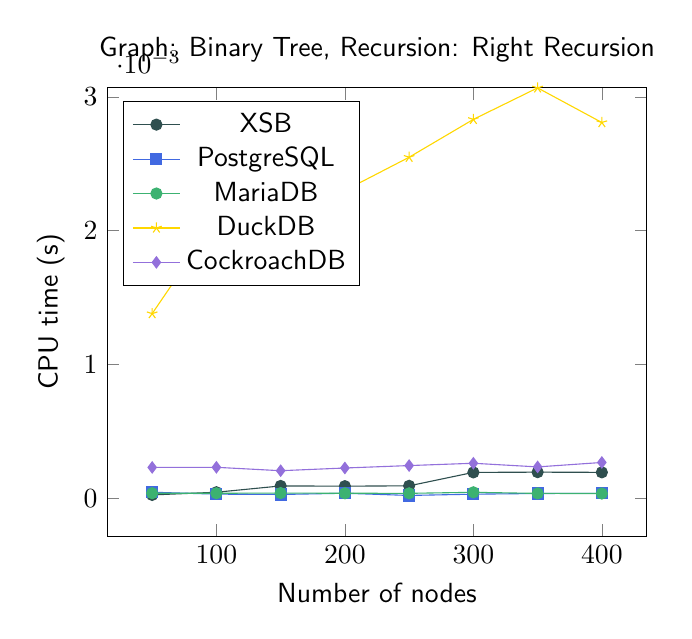
\begin{tikzpicture}
    \begin{axis}[
        title={Graph: Binary Tree, Recursion: Right Recursion},
        xlabel={Number of nodes},
        ylabel={CPU time (s)},
        legend pos={north west},
        ymax=0.003066799999999992
    ]
    \addplot+[DarkSlateGray, mark options={color=DarkSlateGray}] coordinates {(50,2.5599999999999918e-05) (100,4.5800000000000016e-05) (150,9.279999999999983e-05) (200,9.119999999999998e-05) (250,9.360000000000062e-05) (300,0.00019400000000000022) (350,0.0001958000000000004) (400,0.0001944)};
\addlegendentry{XSB}
\addplot+[RoyalBlue, mark options={color=RoyalBlue}] coordinates {(50,4.579999999999584e-05) (100,3.16000000000205e-05) (150,2.8999999999990144e-05) (200,3.819999999999934e-05) (250,2.1799999999982945e-05) (300,3.11999999999979e-05) (350,3.64000000000142e-05) (400,3.76000000000154e-05)};
\addlegendentry{PostgreSQL}
\addplot+[MediumSeaGreen, mark options={color=MediumSeaGreen}] coordinates {(50,3.8600000000010845e-05) (100,3.819999999998824e-05) (150,3.939999999997834e-05) (200,3.8000000000026904e-05) (250,3.7600000000004295e-05) (300,4.5200000000000794e-05) (350,3.699999999997594e-05) (400,3.619999999998624e-05)};
\addlegendentry{MariaDB}
\addplot+[Gold, mark options={color=Gold}] coordinates {(50,0.001380199999999998) (100,0.0020838000000000024) (150,0.002083999999999997) (200,0.0023005999999999973) (250,0.0025486000000000232) (300,0.002831400000000006) (350,0.003066799999999992) (400,0.0028080000000000106)};
\addlegendentry{DuckDB}
\addplot+[MediumPurple, mark options={color=MediumPurple}] coordinates {(50,0.00023120000000000917) (100,0.00023199999999998778) (150,0.00020660000000001234) (200,0.00022680000000000478) (250,0.00024500000000000633) (300,0.00026220000000001244) (350,0.00023499999999998522) (400,0.0002681999999999962)};
\addlegendentry{CockroachDB}

    \end{axis}
\end{tikzpicture}
\end{document}
